% ==============================================================================
% core_step5_pid.tex — SCI/SICE tutorial core deck, Step 5: PID (exercise 8,
% checked in SILS). Only the parallel form is used (no other PID forms).
% The block diagram is drawn inline because the shared pid_block figure uses
% the other (Ti/Td) notation.
% SCI/SICE チュートリアル要点版 Step 5: PID（実習 8、SILS で確認）。
% 並列形だけを使う。共有の pid_block 図は別の記法（Ti/Td）なので、
% ブロック図はここで描く。
% ==============================================================================

% ------------------------------------------------------------------
\begin{frame}{PID 制御器の構成（並列形）}
  \begin{columns}[c]
    \begin{column}{0.60\textwidth}
      \centering
      \adjustbox{max width=\columnwidth, max height=0.50\textheight}{%
      \begin{tikzpicture}[
          blk/.style={rectangle, draw=sfdark, line width=1pt, fill=sflight,
                      rounded corners=2pt, minimum width=20mm, minimum height=9mm},
          sm/.style={circle, draw=sfdark, line width=1pt, fill=white, inner sep=0pt,
                     minimum size=4mm},
          arr/.style={-{Stealth[length=1.6mm,width=1.3mm]}, line width=0.5pt, draw=sfdark},
        ]
        \node[blk] (P) at (30mm, 12mm) {$K_p$};
        \node[blk] (I) at (30mm, 0)    {$K_i/s$};
        \node[blk] (D) at (30mm,-12mm) {$K_d\,s$};
        \node[sm]  (S) at (62mm, 0) {};
        \fill (10mm,0) circle (0.9pt);
        \draw (0,0) -- (10mm,0);
        \draw[arr] (10mm,0) -- (I.west);
        \draw[arr] (10mm,0) |- (P.west);
        \draw[arr] (10mm,0) |- (D.west);
        \draw[arr] (P.east) -| (S.north);
        \draw[arr] (I.east) -- (S.west);
        \draw[arr] (D.east) -| (S.south);
        \draw[arr] (S.east) -- (76mm,0);
        \node[anchor=south] at (4mm,1mm) {$e$};
        \node[anchor=south] at (73mm,1mm) {$u$};
        \node[font=\scriptsize,anchor=south] at (57mm,0.8mm) {$+$};
        \node[font=\scriptsize,anchor=west] at (63mm,6mm) {$+$};
        \node[font=\scriptsize,anchor=west] at (63mm,-6mm) {$+$};
      \end{tikzpicture}}
    \end{column}
    \begin{column}{0.37\textwidth}
      \footnotesize
      \setlength{\abovedisplayskip}{2pt}\setlength{\belowdisplayskip}{2pt}%
      \[ C(s)=K_p+\frac{K_i}{s}+K_d\,s \]
      $e$: 誤差（目標角速度 $-$ ジャイロ）、$u$: ミキサへの指令

      \vspace{0.3em}
      \centering\scriptsize
      実習 8 の解答のゲイン\\[1pt]
      \begin{tabular}{lccc}
        \hline
        & $K_p$ & $K_i$ & $K_d$ \\
        \hline
        Roll  & 0.25 & 0.3 & 0.005 \\
        Pitch & 0.36 & 0.3 & 0.005 \\
        Yaw   & 2.0  & 0.5 & 0.01 \\
        \hline
      \end{tabular}\\[1pt]
      Roll/Pitch の $K_p$ は $\zeta=0.7$ の設計値、Yaw は $\zeta\approx0.88$ 相当
    \end{column}
  \end{columns}

  \vspace{0.3em}
  \begin{itemize}\footnotesize\setlength{\itemsep}{1pt}
    \item \textbf{P}: 今の誤差に比例して押し戻す。一定の外乱トルク（重心のずれ・推力差）に対しては偏差が残る
    \item \textbf{I}: 誤差の積み重ねで押す。一定の外乱に対する偏差を消す。積分値を $\pm0.5$ で打ち切る（アンチワインドアップ: 飽和中に積分が溜まり続けるのを防ぐ）
    \item \textbf{D}: 誤差の変化の速さに比例して押す。行き過ぎ（オーバーシュート）を抑える
  \end{itemize}
\end{frame}

% ------------------------------------------------------------------
\begin{frame}[fragile]{実習 8: PID を実装する}
  \exgoal{実習 5 の P 制御に I 項・D 項を足し、改善を確かめる}
  \begin{columns}[T]
    \begin{column}{0.44\textwidth}
      {\footnotesize\textbf{\textcolor{sfblue}{手順}}}\par\vspace{-2pt}
        \footnotesize
        \begin{enumerate}\setlength{\itemsep}{0pt}
          \item \code{sf lesson switch sci2026:8}
          \item \code{sf lesson edit} で 3 軸に I・D 項と打ち切りを足して保存
          \item \code{sf lesson build}
          \item 実機の飛行は講師が行う
        \end{enumerate}
    \end{column}
    \begin{column}{0.54\textwidth}
      \begin{sflisting}[basicstyle=\ttfamily\scriptsize, moredelim={[is][\bfseries\color{sfred}]{<<}{>>}}]{user\_code.cpp（Roll 軸）}
<<static float integral = 0, prev_err = 0;>>
if disarmed: <<integral = prev_err = 0;>>
float err = target - ws::gyro_x();
<<integral += err * dt;>>
<<integral = clamp(integral, 0.5f);>>
<<float u = Kp*err + Ki*integral>>
<<  + Kd*(err - prev_err)/dt;>>
<<prev_err = err;>>
<<roll_out = clamp(u, 1.0f);>>
      \end{sflisting}
    \end{column}
  \end{columns}
  \exresult{実習 5（P のみ）より行き過ぎが抑えられる（SILS で確認）}
  \exhelptodo{8}
\end{frame}

% ------------------------------------------------------------------
\begin{frame}[fragile]{実習 8 を SILS で確認する}
  \exgoal{書いたコードを PC 上で飛ばし、ソフトの誤り（状態遷移の抜け、発散）がないか確かめる}
  \begin{columns}[T]
    \begin{column}{0.52\textwidth}
      {\footnotesize SILS（Software In the Loop Simulation）: 実機と同じファームのソースを PC で動かし、物理シミュレータと閉ループでつなぐ。墜落の心配なく試せる\par}\vspace{2pt}
      {\footnotesize\textbf{\textcolor{sfblue}{手順（全員、実機は不要）}}}\par\vspace{-2pt}
      \footnotesize
      \begin{enumerate}\setlength{\itemsep}{0pt}
        \item 自分のコードのまま \code{sf lesson sils}
        \item 書き切れなかった人は先に \code{sf lesson switch sci2026:8 --solution}
      \end{enumerate}
    \end{column}
    \begin{column}{0.44\textwidth}
      \begin{sflisting}[basicstyle=\ttfamily\scriptsize]{コマンド}
sf lesson sils
      \end{sflisting}
      \begin{exampleblock}{期待結果: PASS}
        \scriptsize \code{workshop\_acro.expect} で判定: ログに ARM accepted、Takeoff detected、Takeoff complete、DISARM accepted がこの順に出る、高度 $>0.1$\,m、傾き $15^\circ$ 未満
      \end{exampleblock}
      {\scriptsize \code{--scenario step}: ステップ入力のシナリオ（\code{.expect} の合否判定はなく、応答を見る用）。\code{sf sils gui} は機体本体のファーム向けで、実習コードでは未確認\par}
    \end{column}
  \end{columns}
\end{frame}

% ------------------------------------------------------------------
\begin{frame}[fragile]{期待結果: P と PID のロールのステップ応答}
  \begin{center}
    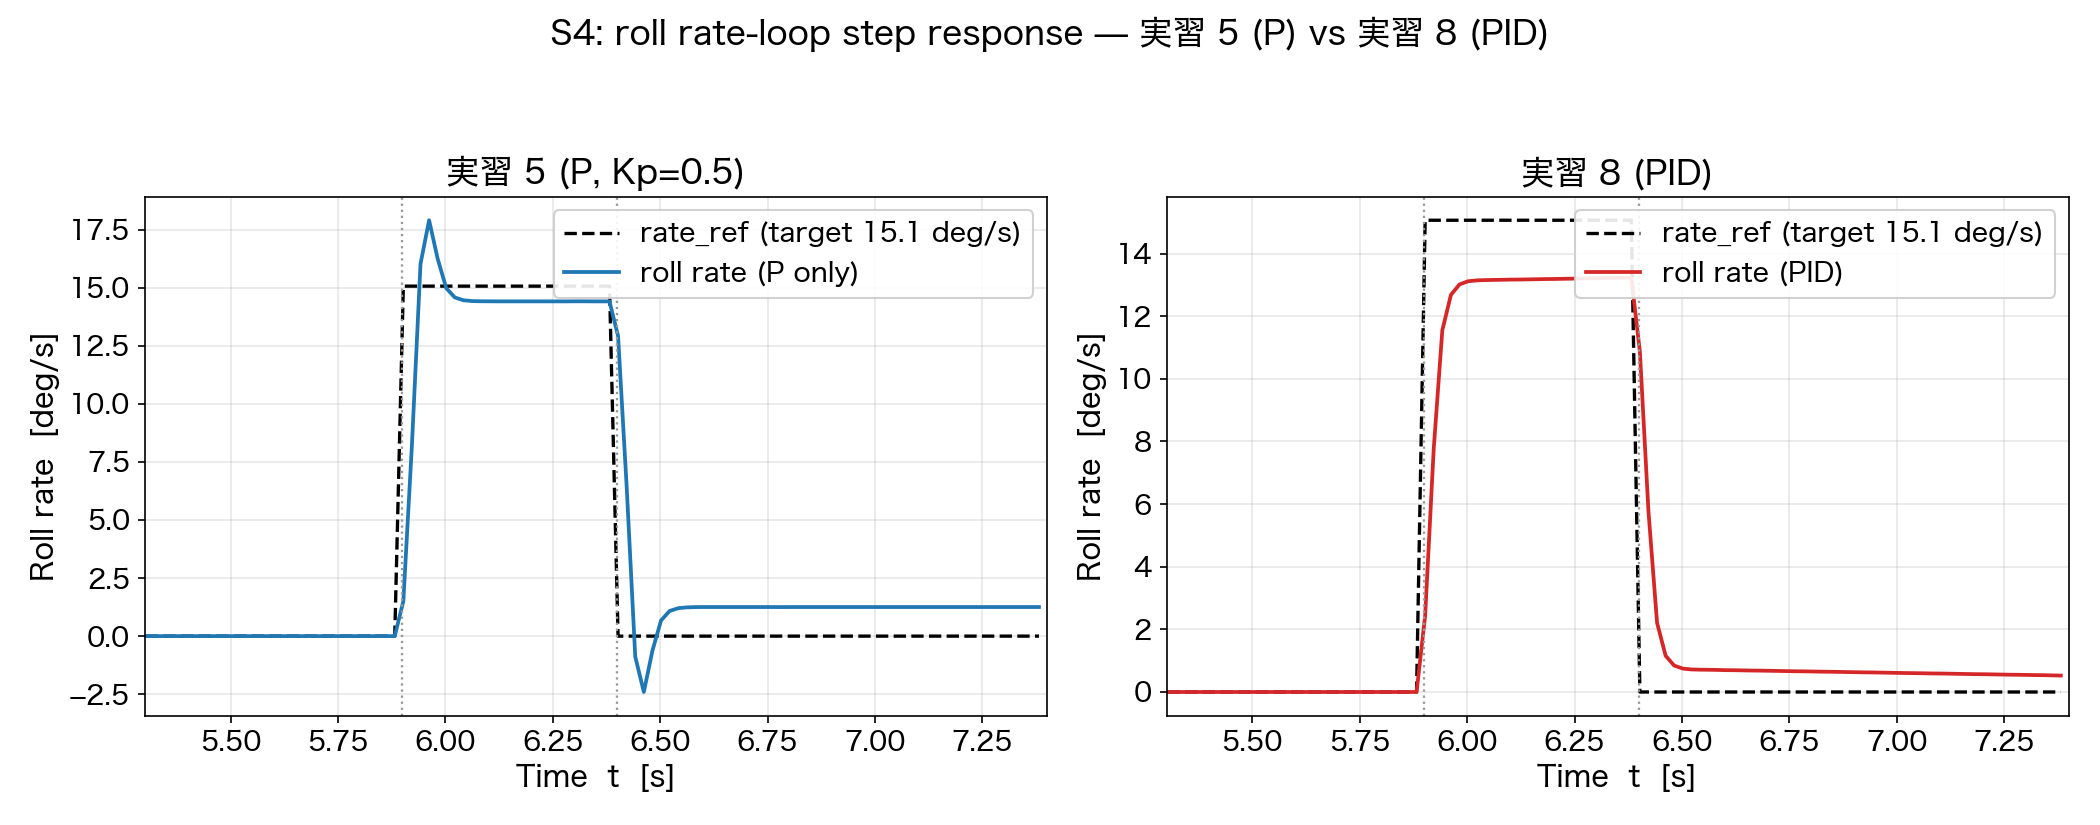
\includegraphics[width=0.94\textwidth, height=0.44\paperheight, keepaspectratio]{../fallback/S4_roll_step_p_vs_pid.png}
  \end{center}
  \vspace{-0.3em}
  \begin{itemize}\footnotesize\setlength{\itemsep}{0pt}
    \item 実習 5（P）: 目標 15.1\,deg/s に対しピーク 17.9\,deg/s の行き過ぎ。指令を戻すと $-2.4$\,deg/s まで振れ、$+1.3$\,deg/s が残る
    \item 実習 8（PID）: 行き過ぎや振動がなく、立ち上がりはゆるやか
  \end{itemize}
  {\scriptsize SILS（MuJoCo）、ロール指令 $+0.3$ を 0.5\,s。再現: \code{sf lesson switch sci2026:8 --solution}、\code{sf lesson sils --scenario step}\par}
\end{frame}
